% \setcounter{chapter}{3}
\chapter{Chapitre 2 - L'analyse multidimensionnelle par réseau de co-expression de gènes}
% \chapter*{Chapitre 2 - L'analyse multidimensionnelle par réseau de co-expression de gènes}
% \phantomsection\addcontentsline{toc}{chapter}{Chapitre 2 - À définir} 
%%\chapter{Titre du chapitre}     % numéroté
\label{chapter:multidim}

\section{Introduction}

La variation de la distribution de la co-expression des gènes associée au vieillissement est une propriété qu'on a pu observer dans le muscle lors du chapitre précédent. Grâce à elle, on a pu isoler dans le chapitre précédent des gènes dont la fonction physiologique est confirmée comme liée au vieillissement du muscle. On peut alors considérer l'étude de la topologie des réseaux de co-expression de gènes comme une méthode efficace pour la détection de gènes biomarqueurs du vieillissement dans un tissu. 

Cependant le vieillissement est un phénomène qui ne se limite pas au muscle dans un organisme et touche bien d'autres tissus en parallèle. Dans chacun d'eux, le transcriptome est le témoin des modifications liées à l'avancée dans l'âge. Comme souligné en introduction (voir \ref{intro_biomarker_aging}), l'analyse d'expression différentielle ainsi que d'autres méthodes d'analyse de gènes discrètes \cite{Barabasi2004} ont permis de relever nombre de gènes (biomarqueurs) associés à l'âge et de créer des bases de données les regroupant. 

Si certains de ces gènes ont déjà vu étudié les liens les unissant dans des fonctions physiologiques, ce n'est pas le cas de la majorité. Ce manque est dû aux méthodes longues et/ou couteuses d'obtention de ces informations qui requièrent notamment des expérimentation basées sur des inactivation ou sur-activation \todo{La traduction dans le grand dico du québec c'est "invalidation" mais y'a rien pour knock in. Et puis c'est moins parlant je trouve.} d'un ou plusieurs gènes (respectivement \textit{knockout} et \textit{knockin} en anglais). 
L'information apportée par de tels liens permettrait pourtant d'aider à déterminer le type de modification observé \cite{Lopez-Otin2013} : l'activation/répression du gène observé est-elle le fruit d'une réponse à l'activation d'un autre gène voir mécanisme complet ? Ou bien est-elle à l'origine d'un mécanisme justement, avec ou sans autres gènes impliqué ? 

Ces questions (qu'on peut résumer à "conséquence ou cause") ont d'autant plus d'intérêt que des études précédentes tendent à démontrer l'existence de bases communes au vieillissement (fonctions physiologiques et mécanismes) \cite{DeMagalhaes2009a}. On relève ainsi des signatures d'expression de gènes communes à plusieurs tissus dans leur état "âgé". Parmi les fonctions physiologiques détectées comme sur-exprimées par l'expression différentielle, on retrouve notamment des composantes de la réponse immunitaire/inflammatoire et de la dégradation lysosomale. À l'opposé, dans les fonctions détectées comme sous-exprimées, on retrouve des fonctions associées à l'encodage de protéines mitochondriales ainsi que des gènes responsables de la production de différents types de collagène. En complément, bien que n'étant pas commun à tous les tissus du corps, d'autres signatures sont communes à des sous groupes de tissus partageant des propriétés : accumulation de marques de réparation de l'ADN chez les tissus se renouvelant rapidement \cite{Armanios2012}, épuisement des capacités de régénération chez les tissus disposant d'une cache de cellules souches \cite{Ratajczak2017}, dommages à l'ADN plus présents chez les tissus soumis à des stress mécaniques \cite{Kubben2017}, etc.

L'analyse de co-expression de gènes ayant déjà démontré sa capacité à aider à la détermination de nouveaux liens, de nouvelles voies de signalisation dans un tissu \cite{Hughes2000}, on souhaite l'employer pour créer des liens entre tissus. Dans ce chapitre, on s'attachera donc à déterminer si l'analyse par réseaux de co-expression de gènes permet de répondre à ce besoin \todo{Peut etre reformuler pour que ça fasse plus hypothès/problématique}. On commencera par traiter les données issues de différents tissus tout en expliquant les précautions prises, on poursuivra par l'exploration générale des modules de gènes obtenus, et enfin on s'attardera sur les apports du croisement de données entre modules modérément préservés (MP) et/ou non préservés (NP). \todo{Reverifier plus tard si ce plan tient toujours, notamment si on a pas rajouté un aspect etude de la déconnexion}

% Objectif principal : 
% Étudier la variation de la déconnexion entre les tranches d'âge extrêmes 
% dans de multiples tissus

% Objectifs secondaires :

% * Vérifier le nombre d'échantillons par tranche d'âge de 10 ans
% * Identifier les tissus d'intérêt pour explorer la déconnexion.
% * Détecter les modules avec chute de connectivité.
% * Déterminer les gènes communs et les gènes spécifiques, et leurs interactions.
% * Explorer les modèles de déconnexion entre les tissus.

% \section{Données et pré-traitement}
\section{Matériel et méthodes}

\subsection{Contextualisation des données}

Comme dans le chapitre \ref{chapter:gwena}, on a utilisé les données issues de l'étude GTEx \cite{Ardlie2015}. Pour aller plus en détail que ce que ne le permet le format d'article du chapitre \ref{chapter:gwena}, ces données sont le regroupement d'échantillons prélevés sur 54 tissus (+1 tissu qui est en fait un assemblage de lignées cellulaires dérivées de patients atteints de leucémie myéloïde aiguë\cite{Way2020}) et 948 donneurs dans sa dernière version, la v8 (Table \ref{table:gtex_sample_tissues_donnor}. Cette variété de tissus vise à être le plus représentatif possible (au vu du coup de prélèvement et d'analyse de chaque échantillon) des différents tissus chez l'humain. Les biopsies sont effectuées sur des donneurs décédés (avec leur accord préalable, l'accord d'un proche, ou l'accord du représentant légal) dans 4 centres de collecte, puis analysées sur place ou transférées selon le tissu avec réfrigération durant le transport. Ces échantillons sont évalués sur plusieurs critères pour jauger leur admissibilité : des critères cliniques (absence de contamination au VIH, absence de chimiothérapie dans les 2 ans, absence de transfusion sanguine dans les 48h, etc.), des critères anatomopathologiques (absence de tissu cancéreux, absence de pathologie tissulaire, etc.) et des critères analytiques (quantité de tissu prélevé suffisante, quantité d'ARN extrait final supérieur à 500ng d'ARN total, nombre d'intégrité d'ARN ou RIN supérieur à 5.7) \cite{Carithers2015}. Tout échantillon non conforme est exclu de la cohorte.

Sur la majorité intégralité des échantillons ont été effectué des séquençages de génome (\textit{Whole Genome Sequencing}, WGS), des séquençages d'exome complet (\textit{Whole Exome Sequencing}, WES), des séquençage de transcriptome (aussi appelé séquençage d'ARN, RNA-Seq), ainsi que des des images de coupes histologiques colorées. Des données reformatées sont également mises à disposition telle que les locus de caractères quantitatifs (\textit{quantitative trait loci}, QTL) et l'expression de gène qui est ce que l'on va utiliser ici. Ces données sont disponibles sur le site du consortium GTEx (\url{https://gtexportal.org}) accompagnées d'information sur le phénotype des échantillons. En raison du fort potentiel d'identification des donneurs, le phénotype donné publiquement est partiel, et le phénotype complet est disponible sur demande auprès de dbGaP après soumission d'un dossier de projet à renouveler chaque année (Annexe \ref{annexe:dbgap}).

\begin{table}[h]
\centering
\begin{tabular}{llll}
\textbf{GTEx V8} & \textbf{\# Tissus} & \textbf{\# Donneurs} & \textbf{\# Échantillons} \\ \hline
Total            & 54                 & 948                  & 17382                    \\
Avec Genotype    & 54                 & 838                  & 15253                    \\
Avec eQTL        & 49                 & 838                  & 15201                   
\end{tabular}
\caption{Nombre de tissus, donneurs et échantillons disponibles selon les données}
\label{table:gtex_sample_tissues_donnor}
\end{table}

Par ailleurs, tous les donneurs n'ont pas pu être prélevés pour l'ensemble des 54 tissus et ce sont en moyenne 23,4 tissus qui ont été prélevés (v8). Certains tissus ont été priorisés lors des biopsies : tissu adipeux (sous-cutané), artère tibiale, coeur (ventricule gauche), poumon, muscle (squelettique), nerf tibial, peau (exposée au soleil), thyroïde, sang complet. Parmi les différents tissus biopsiés, il est à noter que certains sont issus d'un même organe et on a ainsi 31 organes biopsiés pour 54 tissus biopsiés en tout (Figure \todo{faire une figure avec cette info}).

\todo[inline]{Un Sankey diagramme des tissus avec col 1 = SMTS, col 2 = SMTSD, col 3 = tranche d'age à 10 ans}


\subsection{Sélection des tissus}

\todo[inline]{Faire une figure avec l'évolution de la disparition du nombre de tissus}

Le vieillissement est un phénomène dont les altérations moléculaires sont linéaires avec le temps, dont les dommages cellulaires sont super-linéaires \cite{Todhunter2018}, et où la mortalité associée augmente de façon exponentielle passé 20 ans \cite{Finch2016}. Afin de faciliter la détection de ces altérations grâce à l'analyse de co-expression différentielle, on s'est donc dans un premier temps concentré sur une sélection de tranches d'âges très contrastées. Les échantillons sélectionnés sont issus de donneurs entre 20 et 30 ans pour la tranche qu'on nommera "\textbf{jeune}", et entre 60 et 70 ans pour la tranche qu'on nommera "\textbf{âgée}". Les données de GTEx ne comportent toutefois pas un nombre d'échantillons similaire pour chacune de ces tranches du fait de la mortalité plus importante chez les personnes âgées que les personnes jeunes (principalement des décès par traumatisme chez les jeunes plutôt que par maladie chronique ou maladie liée à l'âge chez les âgés). Un premier filtre de notre pré-traitement restreint donc la sélection des tissus à ceux comportant au minimum 50 échantillons dans chacune des tranches d'âge, ce qui n'est pas le cas de la Vessie (20) et le Rein - Médulla (3). Ce nombre d'échantillons permet d'assurer un bon compromis entre des réseaux de co-expression de gènes robustes (donc non sensibles à des valeurs aberrantes) et la perte de plus de tissus à étudier dans cette analyse multidimensionnelle qu'on souhaite effectuer \cite{Liesecke2019}.

Tous les tissus restant n'étaient pas nécessairement adaptés à l'étude globale du vieillissement chez l'humain. Ainsi on a retiré tous les tissus liés à un seul sexe : Trompes de Fallope, Col de l'utérus, Utérus, Vagin, Sein, Ovaire, Prostate, Testicule. À ce retrait s'ajoute celui des échantillons de lignées cellulaires (dérivées ou non de tissus eux concervés) car non représentatifs du vieillissement biologique : Cellules - Lymphocytes transformés par EBV, Cellules - Fibroblastes cultivés, Cellules - Lignée cellulaire de leucémie (CML). 


\begin{figure*}[h]
    \centering
    \includegraphics[width=1\textwidth]{img/chap2/chap2_sample_count_by_tissu.png}
    \label{figure:sample_count_by_tissu}
    \caption{Nombre d'échantilllons disponibles par tissu et par tranche d'âge de 10 ans dans les données de GTEx.}
\end{figure*}


\subsection{Filtre des échantillons}

\todo[inline]{Faire une figure avec l'évolution de la disparition du nombre d'échantillons. Ou bien faire du 2 en 1 avec la précédente sur les selections de tissus ?}

En plus de ces sélections de tissus, certains échantillons ont directement nécessité une filtration afin de prévenir de potentiels biais. Ainsi, seuls les échantillons répondant au critère d'inclusion dans la cohorte "GTEx Analysis Freeze" ont été retenus en premier lieu. Cette cohorte atteste que les échantillons n'étaient pas issus de donneurs ayant des liens de parenté ou de donneurs avec des critères d'exclusion, par exemple des donneurs avec des duplications/déletions chromosomiques, affectés d'un syndrome tel que défini par la base de données OMIM \cite{Hamosh2005} (ce qui n'inclue pas les maladies liées au vieillissement), ou encore ayant effectué une chirurgie de ré-assignation sexuelle. 

Par ailleurs, l'expression des tissus tumoraux a montré, dans des études préalables, des modèles d'expression génétique différents de ceux non tumoraux \cite{Tang2017}. Par conséquent, les échantillons de ces donneurs on également été supprimées ici ainsi que les échantillons dont le statut cancéreux était inconnu. 


\subsection{Correction des facteurs confondants}

À l'instar de l'analyse d'expression différentielle, l'analyse de co-expression différentielle nécessite des données biaisées au minimum pour une construction de réseau de qualité. Ces biais (ou facteurs confondants) peuvent être tant techniques que biologiques et vont entraîner une augmentation de la variation de façon artificielle. Le risque est alors de détecter une différence artificielle et de l'assumer comme expérimentalement pertinente alors qu'elle est en fait due aux biais. Dans le cas de la co-expression plus spécifiquement, ces bais peuvent entraîner des corrélations erronées mais qui semblent crédibles entre certains gènes. Elles altèrent alors la construction du réseaux de co-expression et par la suite la détection des modules qui se base sur un découpage en modules via les corrélations. Ainsi, il est essentiel de corriger ces facteurs confondants au préalable de l'utilisation du package R GWENA \todo{REF} sur les données comme on va le faire par la suite.

La complexité de la correction des facteurs confondant réside dans leur suppression sans pour autant altérer la distribution des données ou supprimer le signal expérimental d'intérêt, ici les variations dans le transcriptome dûs à l'âge. Il est également important avec l'utilisation de GWENA de veiller à ce que la correction n'altère pas la topologie d'invariance d'échelle qu'on retrouve dans les données de transcriptomique après construction d'un réseau de co-expression. En effet, cela invaliderait la méthode de détection des modules.
% Comme précisé en \ref{subsubsection:microarray_props_and_normalisation} et \ref{subsubsection:rnaseq_props_and_normalisation}, chaque technologie de séquençage a un premier ensemble de normalisations spécifique à elle, limitant ainsi un premier ensemble de biais spécifiques. 
\todo{Je me demande si ces 2 paragraphes plus haut ne devraient pas finir en intro de thèse}

La base de données GTEx n'échappe pas aux biais et a même été étudiée sur le plan de la contamination \cite{Nieuwenhuis2020}.
Malgré le progrès de techniques ciblées sur des facteurs confondants connus comme l'effet de lot, l'effet de centre de prélèvement, le sexe, le poids, etc., celles-ci ne sont pas capables de corriger pour des facteurs peu explicites ou diffus comme la classe sociale, l'alimentation, la façon de manipuler des techniciens, etc. La correction par composante principale (CP) vise à répondre à ce type de problématique et a montré de bons résultats selon une évaluation par validation de pathways au sain de modules détectés. \cite{Parsana2019}. Elle a également montré de meilleurs résultats que d'autres méthodes telles que que la régression multiple, le taux exonique, ou encore le numéro d'intégrité d'ARN (\textit{RNA integrity number}, ou RIN). Fait important pour la co-expression en particulier, cette méthode conserve la propriété d'invariance d'échelle des données.

Cependant cette correction va également corriger l'âge qui est notre variable d'intérêt. Afin de conserver cette information tout en ayant un effet de correction par CP suffisant, on a ajusté le nombre $n$ de CP par lequel corriger les jeux de données. L'estimation de $n$ s'est faite en deux étapes :
\begin{itemize}
    \item Un test de corrélation de chaque gene avec l'âge associé à chaque échantillon en fonction de différent $n$ PC corrigées donne une liste de gènes significativement associés à l'âge.
    \item Cette liste de gènes par $n$ PC corrigées est ensuite croisée avec deux bases de données de gènes connus comme étant associés au vieillissement : GenAge \cite{DeMagalhaes2004} et Digital Aging Atlas \cite{Craig2015}. Y sont alors compté le nombre de gènes significatifs recoupés.
\end{itemize}
Finalement, le $n$ de PC à corriger retenu est celui où le nombre de gènes significatifs est le plus haut dans chaque base de données. En cas de divergence de ce $n$ entre les bases de données, on a sélectionné la valeur la plus basse de $n$ afin de ne pas risquer de corriger l'âge (Table \ref{table:nb_PC_corr_and_samples_by_tissue}).


\begin{table}[h!]
% \resizebox{\textwidth}{!}{
\centering
\begin{tabular}{llll}
\multirow{2}{*}{\textbf{Tissu}} & \multirow{2}{*}{\textbf{\begin{tabular}[c]{@{}l@{}}Nombre de CP \\ corrigées\end{tabular}}} & \multicolumn{2}{l}{\textbf{Nombre d'échantillons}} \\ \cline{3-4} 
                                &                                                                                             & \textbf{Jeune}            & \textbf{Âgé}           \\ \hline
Adipeux sous-cutané             & 1                                                                                           & 58                        & 227                    \\
Artère tibiale                  & 3                                                                                           & 65                        & 206                    \\
Muqueuse œusophagienne          & 1                                                                                           & 59                        & 160                    \\
Muscle œusophagien              & 3                                                                                           & 64                        & 138                    \\
Muscle squelettique             & 5                                                                                           & 73                        & 281                    \\
Nerf tibial                     & 4                                                                                           & 56                        & 219                    \\
Peau non exposée au soleil      & 4                                                                                           & 50                        & 220                    \\
Peau exposée au soleil          & 3                                                                                           & 65                        & 250                    \\
Thyroïde                        & 3                                                                                           & 53                        & 227                    \\
Sang complet                    & 1                                                                                           & 73                        & 259                   
\end{tabular}
% }
\caption{Résumé du nombre de composantes utilisées pour effectuer la correction de l'expression par tissu, ainsi que le nombre d'échantillons inclus dans chacun pour les deux plages d'âge.}
\label{table:nb_PC_corr_and_samples_by_tissue}
\end{table}

\todo[inline]{Idée de figure : remplacer cette table ou en touts cas la partie nb composantes par un ensemble de mini histogrames avec les deux bdd en un, et en facet pour chaque tissu.}

\subsection{Filtre sur les gènes}

On a considéré comme base dans cette étude uniquement les gènes codants pour une protéine (d'après GENCODE 26) sur les autosomes ainsi que le chromosome X (toujours dans cette idée de ne pas avoir l'influence d'un sexe). Afin de limiter l'ajout de biais d'origine technique, on a également exclu les gènes dont le compte de lecture (en anglais \textit{count})  était inférieur à 6 \cite{Rocke2001}. Les gènes n'ayant aucune variation se sont vu retirés du jeu de données car leur apport à la co-expression aurait était nul et leur conservation aurait entraîné l'utilisation de ressources inutile.



% \section{Construction des réseaux par tissu et détection des modules}
% \section{Isolement des modules d'intérêt}
\section{Résultats}

% Suite à ce pré-traitement des données, on a pu s'attacher 
% \subsection{Construction des réseaux par tissu et détection des modules}
En utilisant les données d'expression qui ont passé les contrôles de qualité décrits ci-dessus, nous avons généré un réseau de co-expression de gènes indépendemment sur chacun des 10 tissus et tranche d'âge à l'aide du package GWENA. 
% La loi de puissance associée à chacun des réseau a retourné des \textalpha 
% \begin{table}[h]
% \centering
% \begin{tabular}{lll}
% \textbf{Tissu}             & \textbf{\textalpha  Jeune} & \textbf{ \textalpha  Âgé} \\ \hline
% Adipeux sous-cutané        & 14             & 14           \\
% Artère tibiale             & 6              & 9            \\
% Muqueuse œusophagienne     & 14             & 16           \\
% Muscle œusophagien         & 12             & 18           \\
% Muscle squelettique        & 6              & 8            \\
% Nerf tibial                & 7              & 12           \\
% Peau non exposée au soleil & 8              & 8            \\
% Peau exposée au soleil     & 10             & 10           \\
% Thyroïde                   & 16             & 12           \\
% Sang complet               & 18             & 14          
% \end{tabular}
% \end{table}
Dans chaque réseau, on a ensuite détecté le nombre de modules optimaux (à seuil de coupe identique de l'arbre hiérarchique) avec une variation de leur nombre visible en Figure \ref{figure:repartition_genes_modules_tissus} entre couples tissus / tranche d'âge.

\begin{figure}[hb]
    \centering
    \includegraphics[width=1\textwidth]{img/chap2/chap2_repartition_genes_modules_tissus.png}
    \caption{Répartition des gènes (en échelle log10) pour chaque tissu entre les deux tranches d'âge jeune (bleu) et âgée (rouge)}
    \label{figure:repartition_genes_modules_tissus}
\end{figure}

On constate que la répartition des gènes entre les modules est hétérogène, tant entre les tranches d'âge qu'entre les tissus, avec une moyenne à 26 modules tout confondu (25.2 pour les âgés et 26.8 pour les jeunes). Le module 0 présent sur la figure regroupe les gènes sans association à un module. Celui-ci est quasi systématiquement plus grand dans la tranche âgée que jeune, à l'exception des tissus de la thyroïde et du sang complet. Les tissus où cet écart est le plus creusé sont ceux disposant du plus grand nombre de modules dans la tranche d'âge jeune. Ces résultats sont cohérents avec la tendance à la perte de co-expression constatée dans les tranches d'âge âgées \cite{Southworth2009} : la perturbation des voies de signalisation au cours du vieillissement entraîne une diminution de la co-expression entre gènes de ces voies.

\subsection{Modules spécifiques du vieillissement et recoupement inter-tissus}

% Le but étant de rechercher les origines des gènes associés au vieillissement 
Le but étant de rechercher des origines communes au vieillissement entre tous les tissus, on a ensuite effectué une étape de co-expression différentielle intra tissu. La tranche d'âge jeune a été prise pour référence, c'est à dire que le test indiquera si chaque module détecté dans la tranche d'âge jeune est préservé, modérément préservé, non préservé, ou non concluant. Les résultats on été résumés en Table \ref{table:modules_status_all_tissues}. On y constate que certains tissus tendent à avoir proportionnellement beaucoup moins de modules préservés lors du vieillissement, c'est notamment le cas des muscles œsophagiens et squeletaux, ainsi que de la peau exposée au soleil et la thyroïde. À cela s'ajoute que la peau exposée au soleil et le muscle squelettique sont les deux tissus ayant le plus de modules on préservés directement.

\begin{table}[h]
\resizebox{\textwidth}{!}{
\begin{tabular}{llllllllll}
\multirow{2}{*}{\textbf{Tissu}} & \multicolumn{2}{l}{\textbf{Préservé}} & \multicolumn{2}{l}{\textbf{Modérement préservé}} & \multicolumn{2}{l}{\textbf{Non préservé}} & \multicolumn{2}{l}{\textbf{Non concluant}} & \textbf{Total} \\ \cline{2-10} 
                                & \textbf{\#}       & \textbf{\%}       & \textbf{\#}             & \textbf{\%}            & \textbf{\#}         & \textbf{\%}         & \textbf{\#}          & \textbf{\%}         & \textbf{\#}    \\ \hline
Adipeux sous-cutané             & 12                & 0.67              & 4                       & 0.22                   & 0                   & 0                   & 2                    & 0.11                & 18             \\
Artère tibiale                  & 13                & 0.57              & 8                       & 0.35                   & 1                   & 0.04                & 1                    & 0.04                & 23             \\
Muqueuse œusophagienne          & 3                 & 0.25              & 8                       & 0.67                   & 1                   & 0.08                & 0                    & 0                   & 12             \\
Muscle œusophagien              & 9                 & 0.43              & 6                       & 0.29                   & 0                   & 0                   & 6                    & 0.29                & 21             \\
Muscle squelettique             & 14                & 0.40              & 13                      & 0.37                   & 5                   & 0.14                & 3                    & 0.09                & 35             \\
Nerf tibial                     & 35                & 0.71              & 9                       & 0.18                   & 1                   & 0.02                & 4                    & 0.08                & 49             \\
Peau non exposée au soleil      & 36                & 0.90              & 4                       & 0.10                   & 0                   & 0                   & 0                    & 0                   & 40             \\
Peau exposée au soleil          & 10                & 0.48              & 8                       & 0.38                   & 2                   & 0.10                & 1                    & 0.05                & 21             \\
Thyroïde                        & 12                & 0.48              & 8                       & 0.32                   & 1                   & 0.04                & 4                    & 0.16                & 25             \\
Sang complet                    & 9                 & 0.64              & 4                       & 0.29                   & 0                   & 0                   & 1                    & 0.07                & 14              
\end{tabular}
}
\caption{Nombre (\#) et ratio (\%) de modules par statut de préservation selon chaque tissu.}
\label{table:modules_status_all_tissues}
\end{table}

%  0.64|                   0.29|            NA|           0.07|

Afin d'observer des similarités de mécanismes du vieillissement entre ces différents tissus, on a dans un premier temps regardé si des gènes communs existaient entre les modules modérément préservés (MP) et non  préservés (NP). Le diagramme UpSet visible en Figure \ref{figure:upset_intersection_genes_tissu_unpres_modpres} \todo{Peut être retravailler la figure pour la découper selon le nombre de tissus à l'intersection (de 1 à 5)} permet de constater le faible recouvrement entre les gènes contenus dans les modules MP et NP. Ce diagramme révèle également que le maximum de tissus avec des gènes communs est 5. Ce chiffre est à mettre en contraste avec le fait que les modules créés par GWENA pour un même tissu ne sont pas chevauchant. Un gène classé dans un module ne sera donc pas également classé dans un autre et on aurait pu espérer une intersection au maximum de taille 10 étant donné qu'on dispose de 10 tissus. 


\begin{figure}[hp]
    \begin{adjustbox}{addcode={
        \begin{minipage}{\width}}{
            \caption{Intersections entre tous les jeux de gènes pour chaque couple tissu / statut de préservation. Le diagramme Upset est une représentation qui vise à remplacer une visualisation par diagramme de Venn, ce dernier n'étant pas adaptée à la représentation de plus de 5 catégories \cite{Lex2014}. La matrice d'intersection (en orange) indique quel couple tissu / statut est considéré dans l'intersection (rose si pris en compte, gris si non) et quels sont les autres tissus dans cette intersection (ligne rose). L'histogramme des tailles de groupe (gris) à gauche de la matrice indique le nombre total de gène contenu dans le couple tissu / statut en ligne. L'histogramme des tailles d'intersection indique le nombre de gènes contenu dans l'intersection indiquée en matrice d'intersection pour cette colonne.}
        \end{minipage}},rotate=90,center}
        % \includesvg[scale=.5]{img/chap2/chap2_upset_genes_unpres_modpres_by_tissue.svg}
        % \includesvg[width=1\textheight]{img/chap2/chap2_upset_genes_unpres_modpres_by_tissue.svg}
        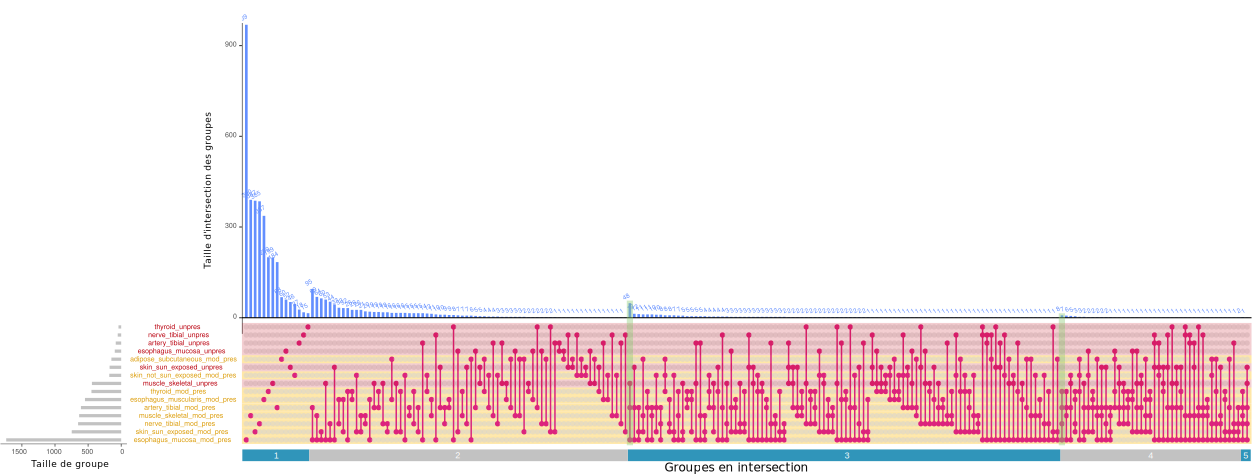
\includegraphics[width=1\textheight]{img/chap2/chap2_upset_genes_unpres_modpres_by_tissue.pdf}
    \end{adjustbox}
    \label{figure:upset_intersection_genes_tissu_unpres_modpres}
\end{figure}


Comme suggéré par les ratios de statut de préservation en table \ref{table:modules_status_all_tissues}, certains tissus tendent à avoir plus de modules MP/NP et/ou des modules de plus grande taille (avec le plus de gènes), favorisant alors leur probabilité de recoupement avec d'autres tissus. Ainsi, les modules MP de la muqueuse œsophagienne regroupent 1750 gènes et tendent à se positionner dans plus d'intersection que la moyenne. Une séparation est toutefois visible entre les deux types de statut MP et NP dans les intersection au delà de 2 tissus et avec un minimum de trois gènes.

\subsection{Répartition des phénomènes communs liés au vieillissement dans plusieurs tissus}

Pour mieux comprendre les fonctions physiologiques communes en jeu et pouvant être impliquées dans le vieillissement, les intersections de plus de 3 tissus et ayant au moins 5 gènes on été enrichies via GWENA. Comme visible en Annexe \ref{annexe:chap_2_genes_intersect_enrichments} dans les tables des enrichissements obtenus, 5 intersections n'ont pas donné d'enrichissement significatif malgré un nombre de gène équivalent à d'autres intersections avec enrichissement. Les 18 autres intersections ont quant à elles retourné des fonctions physiologiques (Gene Ontology \cite{Ashburner2000}, CORUM \cite{Ruepp2008}) et voies d'activation (KEGG \cite{Kanehisa2019}, REACTOME \cite{Fabregat2016}, WikiPathways\cite{Slenter2018}) connues comme faisant partie du vieillissement global, ou de manifestations spécifiques à plusieurs tissus. Ainsi on retrouve, dans ces intersections de modules peu ou pas préservés dans la tranche âgée, des fonctions associées à l'homéostasie, la régulation de la transcription, la gestion des dérivés réactifs de l'oxygène, l'inflammation, etc. (Table \ref{table:intersection_aging_global_phenomenons} et Figure \ref{figure:revigo_resume_4_enrich}). La muqueuse œsophagienne bien qu'ayant un nombre de gènes plus élevé que les autres tissus ne se retrouve pas sur-représentée dans ces phénomènes observés. Cela indique donc que la majorité de ses gènes se trouvent dans les intersections de faible taille, tant en gènes qu'en nombre de tissus recoupés. Le sang complet, le tissu adipeux sous-cutané, et la peau non exposée au soleil sont eux les tissus les moins présents dans ces intersections avec des phénomènes liés au vieillissement. Le sang complet est notablement absent des intersection avec des phénomènes liés à la coagulation. Les tissus ayant un fort renouvellement (voir en partie \ref{tissu_telomere_effet}) que sont les épithéliums (peau exposée au soleil, artère tibiale, muqueuse œsophagienne) sont porteurs d'un grand nombre de phénomènes, ainsi que la thyroïde et le muscle squelettique. 


\begin{table}[]
\resizebox{\textwidth}{!}{
\begin{tabular}{@{}lllllllllll@{}}
\rotatebox{90}{\textbf{Muqueuse œusophagienne}}   & \rotatebox{90}{\textbf{Artère tibiale}}                      & \rotatebox{90}{\textbf{Thyroïde}}                 & \rotatebox{90}{\textbf{Muscle squelettique}}      & \rotatebox{90}{\textbf{Peau exposée au soleil}}   & \rotatebox{90}{\textbf{Muscle œusophagien}}       & \rotatebox{90}{\textbf{Nerf tibial}}              & \rotatebox{90}{\textbf{Peau non exposée au soleil}} & \rotatebox{90}{\textbf{Adipeux sous-cutané}}      & \rotatebox{90}{\textbf{Sang complet}}             & \textbf{Phénomène du vieillissement observé}       \\ \midrule
\cellcolor[HTML]{F8A102} & \cellcolor[HTML]{F8A102}            &                          & \cellcolor[HTML]{F8A102} &                          &                          &                          & \cellcolor[HTML]{F8A102}   &                          &                          & Homéostasie                               \\
                         & \cellcolor[HTML]{F8A102}            & \cellcolor[HTML]{F8A102} &                          &                          & \cellcolor[HTML]{F8A102} &                          &                            &                          &                          & Régulation de la transcription            \\
\cellcolor[HTML]{F8A102} &                                     & \cellcolor[HTML]{F8A102} & \cellcolor[HTML]{F8A102} &                          &                          &                          &                            &                          &                          & Dérivés réactifs de l'oxygène - peroxydes \\
                         &                                     & \cellcolor[HTML]{F8A102} &                          & \cellcolor[HTML]{F8A102} & \cellcolor[HTML]{F8A102} & \cellcolor[HTML]{F8A102} &                            &                          &                          & Dérivés réactifs de l'oxygène - dGTP      \\
                         &                                     & \cellcolor[HTML]{F8A102} &                          &                          &                          &                          & \cellcolor[HTML]{F8A102}   & \cellcolor[HTML]{F8A102} &                          & Inflammation                              \\
                         &                                     &                          &                          & \cellcolor[HTML]{F8A102} & \cellcolor[HTML]{F8A102} & \cellcolor[HTML]{F8A102} &                            &                          &                          & Désamination                              \\
\cellcolor[HTML]{F8A102} & \cellcolor[HTML]{F8A102}            &                          &                          &                          &                          & \cellcolor[HTML]{F8A102} &                            &                          &                          & Coagulation - plaquettes                  \\
\cellcolor[HTML]{F8A102} & \cellcolor[HTML]{F8A102}            & \cellcolor[HTML]{F8A102} &                          &                          &                          & \cellcolor[HTML]{F8A102} &                            &                          &                          & Coagulation - global                      \\
\cellcolor[HTML]{F8A102} & \cellcolor[HTML]{F8A102}            &                          & \cellcolor[HTML]{F8A102} &                          &                          &                          &                            &                          &                          & Méthylation - folate, B12, selenium       \\
                         &                                     &                          & \cellcolor[HTML]{F8A102} & \cellcolor[HTML]{F8A102} &                          &                          &                            & \cellcolor[HTML]{F8A102} &                          & Méthylation - déméthylase                 \\
\cellcolor[HTML]{F8A102} & \cellcolor[HTML]{F8A102}            &                          & \cellcolor[HTML]{F8A102} &                          &                          &                          &                            &                          & \cellcolor[HTML]{F8A102} & Altération de la MEC                      \\
                         &                                     & \cellcolor[HTML]{F8A102} &                          & \cellcolor[HTML]{F8A102} & \cellcolor[HTML]{F8A102} &                          &                            &                          &                          & Anomalie du taux de glutamine             \\
\cellcolor[HTML]{F8A102} &                                     &                          &                          & \cellcolor[HTML]{F8A102} &                          &                          & \cellcolor[HTML]{F8A102}   &                          &                          & Synthèse de pigment (dont mélanine)      \\
\cellcolor[HTML]{F8A102} & \cellcolor[HTML]{F8A102}            & \cellcolor[HTML]{F8A102} & \cellcolor[HTML]{F8A102} &                          &                          &                          &                            &                          &                          & Anomalie du taux de fer                   \\
\midrule
8                        & 7                                   & 7                        & 6                        & 5                        & 4                        & 4                        & 3                          & 2                        & 1                        & \textbf{Total}                   
\end{tabular}
}
\caption{Phénomènes connus dans le vieillissement et observés dans les intersections de modules MP et NP pour chaque tissu. Les modules MP et NP ont été joints par tissus et les tissus ont été ordonnés par nombre décroissant de phénomènes du vieillissement présent. MEC : Matrice extra-cellulaire.}
\label{table:intersection_aging_global_phenomenons}
\end{table}

% \begin{table}[]
% \resizebox{\textwidth}{!}{
% \begin{tabular}{@{}lllllllllll@{}}
% % \toprule
% \rotatebox{90}{\textbf{Adipeux sous-cutané }}      & \rotatebox{90}{\textbf{Artère tibiale }}           & \rotatebox{90}{\textbf{Muqueuse œusophagienne }}   & \rotatebox{90}{\textbf{Muscle œusophagien }}       & \rotatebox{90}{\textbf{Muscle squelettique }}      & \rotatebox{90}{\textbf{Nerf tibial }}              & \rotatebox{90}{\textbf{Peau non exposée au soleil }} & \rotatebox{90}{\textbf{Peau exposée au soleil }}   & \rotatebox{90}{\textbf{Thyroïde }}                 & \rotatebox{90}{\textbf{Sang complet }}             & \textbf{Phénomène du vieillissement observé}       \\ \midrule
%                          & \cellcolor[HTML]{F8A102} & \cellcolor[HTML]{F8A102} &                          & \cellcolor[HTML]{F8A102} &                          & \cellcolor[HTML]{F8A102}   &                          &                          &                          & Homéostasie                               \\
%                          & \cellcolor[HTML]{F8A102} &                          & \cellcolor[HTML]{F8A102} &                          &                          &                            &                          & \cellcolor[HTML]{F8A102} &                          & Régulation de la transcription            \\
%                          &                          & \cellcolor[HTML]{F8A102} &                          & \cellcolor[HTML]{F8A102} &                          &                            &                          & \cellcolor[HTML]{F8A102} &                          & Dérivés réactifs de l'oxygène - peroxydes \\
%                          &                          &                          & \cellcolor[HTML]{F8A102} &                          & \cellcolor[HTML]{F8A102} &                            & \cellcolor[HTML]{F8A102} & \cellcolor[HTML]{F8A102} &                          & Dérivés réactifs de l'oxygène - dGTP      \\
% \cellcolor[HTML]{F8A102} &                          &                          &                          &                          &                          & \cellcolor[HTML]{F8A102}   &                          & \cellcolor[HTML]{F8A102} &                          & Inflammation                              \\
%                          &                          &                          & \cellcolor[HTML]{F8A102} &                          & \cellcolor[HTML]{F8A102} &                            & \cellcolor[HTML]{F8A102} &                          &                          & Désamination                              \\
%                          & \cellcolor[HTML]{F8A102} & \cellcolor[HTML]{F8A102} &                          &                          & \cellcolor[HTML]{F8A102} &                            &                          &                          &                          & Coagulation - plaquettes                  \\
%                          & \cellcolor[HTML]{F8A102} & \cellcolor[HTML]{F8A102} &                          &                          & \cellcolor[HTML]{F8A102} &                            &                          & \cellcolor[HTML]{F8A102} &                          & Coagulation - global                      \\
%                          & \cellcolor[HTML]{F8A102} & \cellcolor[HTML]{F8A102} &                          & \cellcolor[HTML]{F8A102} &                          &                            &                          &                          &                          & Méthylation - folate, B12, selenium       \\
% \cellcolor[HTML]{F8A102} &                          &                          &                          & \cellcolor[HTML]{F8A102} &                          &                            & \cellcolor[HTML]{F8A102} &                          &                          & Méthylation - déméthylase                 \\
%                          & \cellcolor[HTML]{F8A102} & \cellcolor[HTML]{F8A102} &                          & \cellcolor[HTML]{F8A102} &                          &                            &                          &                          & \cellcolor[HTML]{F8A102} & Altération de la MEC                      \\
%                          &                          &                          & \cellcolor[HTML]{F8A102} &                          &                          &                            & \cellcolor[HTML]{F8A102} & \cellcolor[HTML]{F8A102} &                          & Anomalie du taux de glutamine             \\
%                          &                          & \cellcolor[HTML]{F8A102} &                          &                          &                          & \cellcolor[HTML]{F8A102}   & \cellcolor[HTML]{F8A102} &                          &                          & Synthèse de pigement (dont mélanine)      \\
%                          & \cellcolor[HTML]{F8A102} & \cellcolor[HTML]{F8A102} &                          & \cellcolor[HTML]{F8A102} &                          &                            &                          & \cellcolor[HTML]{F8A102} &                          & Anomalie du taux de fer                   \\ 
% \end{tabular}
% }
% \caption{Phénomènes connus dans le vieillissement et observés dans les intersections de modules MP et NP pour chaque tissu. Les modules MP et NP ont été joints par tissus pour une meilleure lisibilité.}
% \label{table:intersection_aging_global_phenomenons}
% \end{table}

\begin{figure}
    \centering
    \includegraphics[width=1\textwidth]{img/chap2/chap2_revigo_resume_4_enrich.png}
    \caption{Exemple de résumé des enrichissements sur GO pour 4 des intersections par carte proportionnelle. Chaque ensemble de GO terme partageant une ontologie parente commune (selon un score de similarité) est groupé sous une même couleur. Chaque carte présente ici un phénomène connu dans le vieillissement : A. Homéostasie (GO *Biological Process*), B. Régulation de la transcription (GO *Biological Process*), C. Dérivés réactifs de l'oxygène (GO *Molecular Function*), D. Inflammation (GO *Biological Process*) }
    \label{figure:revigo_resume_4_enrich}
\end{figure}

Des anomalies phénotypiques ont été relevée (via enrichissement sur HPO \cite{Kohler2019}) et présentent un lien plus ou moins évident avec les altérations physiologiques précédemment relevées. Aux anomalies du taux de fer détectés dans les fonctions physiologiques coïncident ainsi des phénotypes d'anémie (déficience en taux de globules rouges ou en concentration d'hémoglobine) ou de défaut de coagulation avec hémorragies diverses (epistaxie, saignement gingival, menstruations hors cycle, hémoragie cérébrale). De même, les tissus présentant une altération de la matrice extra-cellulaire (MEC) ont été associés avec des taux élevés de protéine C-réactive et d'anomalies de la fonction exocrine du pancréas ainsi que de malabsorption des lipides et ce qui en découle (stéatorrhée, pancréatite, thrombose veineuse). Ces résultats confirment le lien entre vieillissement et dérèglement progressif de l'homeostasie entrainant en cascade des pathologies de trouble de la coagulation \cite{Franchini2006,Kario1993} et de la dégradation des lipides circulants \cite{Yamamoto2014, Hirschfield2003}. Cependant d'autres résultats semblent moins intuitifs comme dans le cas de pathologies liées au sexe (azoospermie, maladie d'hérédité gonosomale) relevées parallèlement à la déméthylation dans le tissu adipeux, le muscle squelettique, et la peau non exposée au soleil. Ces informations, en l'absence d'erreur technique, semblent continuer de montrer la complexité des relations entre pathologies et vieillissement.

Enfin, on a exploré le vieillissement et son phénomène de perturbation de la régulation de la transcription en évaluant l'enrichissement d'éléments de régulation (MiRTarBase \cite{Chou2018}, TRANSFAC \cite{Matys2006}). L'intersection présentant des phénomènes de coagulation globale est ainsi fortement enrichi en micro ARN (miARN). Ceux contiennent notamment des miARN associés aux 3 gènes de la génération de fibrinogène FGA, FGB, FGG comme détectés lors du chapitre précédent. Quelques autres intersections. Deux facteurs de transcription (FT), HNF1A et HNF1B, sont également significatifs bien que normalement exprimés dans le foie. Cela s'explique par la production de facteurs de la coagulation (dont FGA, FGB, FGG) dans celui-ci et un effet connu de l'altération de production de ces facteurs dans le cadre d'une perturbation de l'expression de HNF1A et HNF1B \cite{Costa2003}. L'intersection associée à l'inflammation quand a elle ne présente qu'un seul miARN agissant ici sur RSAD2, IFI44, OASL, et EPSTI1 présents dans l'intersection. RSAD2 et OASL sont également connus pour être stimulé par des interférons de classe I (\textalpha et \textbeta) qui ont entre autres IRF1 (pour interferon related factor 1) pour FT \cite{Schoggins2011}. Ce facteur IRF1 fait par ailleurs parti de la liste des FT détectés dans cette intersection. On y trouve un large panel d'autres membres de la famille d'IRF (de 1 à 9 à l'exception d'IRF6) dont l'implication dans l'inflammation s'exerce tant dans la réaction innée que acquise \cite{Frisch2020}. Mais tous les FT détectés via enrichissement n'étaient pas des IRF. Bien que n'étant pas directement liés à la régulation des interférons, STAT2 est présent dans la voie de signalisation des interférons \textalpha et \textbeta détecté plus tôt (R-HSA-909733). Le dernier FT identifié, FOXP1, n'est quant à lui pas contenu dans cette voie mais agit sur l'engagement des cellules souches mésenchymateuses et la sénescence au cours du vieillissement \cite{Infante2018} et sur de la régulations d'autres cytokines, l'interleukine 1 et 12 d'après UniprotKB (Q9H334).

\subsection{Les variation de co-expression dans l'intersection liée à l'inflammation}

L'inflammation systémique chronique de faible intensité est une des marques connues du vieillissement \cite{Lopez-Otin2013, Franchini2006}. La complexité des mécanismes d'immunité et d'inflammation rend ce phénomène particulièrement difficile à étudier et les publications actuelles tendent donc à cibler un ou quelques acteurs afin de 
% L'inflammation systémique chronique de faible intensité est une manifestation courante du vieillissement.
% La détection de ces différents phénomènes liée à l'âge ayant été permise par le ciblage 

\begin{figure}[b]
    \centering
    \includegraphics[width=1\textwidth]{img/chap2/chap2_graphs_intersection_plot_adipo_skinnosun_thyr.png}
    \caption{Réseaux de co-expression des gènes de l'intersection associée au phénomène d'inflammation lors du vieillissement entre les deux tranches d'âge. Le réseau est filtré à 0.95 de dissimilarité (sur une échelle de 0 à 1) et 3 tissus sont présentés : tissu adipeux, peau non exposée au soleil, et thyroïde.}
    \label{figure:graphs_intersection_plot_adipo_skinnosun_thyr}
\end{figure}



\subsection{Cas particulier : le vieillissement spécifique à la peau}



\subsection{Variation de la co-expression dans le XXX}
Comme attendu au vu de la littérature, de nombreux enrichissements ont retourné des mécanismes et acteurs de l'inflammation. 




\#\#\#\#\#\#\#\#\#\#\#\#\# TRAVAIL EN COURS \#\#\#\#\#\#\#\#\#\#\#\#\#


% Pourquoi le muscle vieillit vite malgré son faible taux de renouvellement : https://www.ncbi.nlm.nih.gov/pmc/articles/PMC3874224/

% À l'inverse, certains gènes dans les modules MP ou NP ne sont présent que dans leur tissu. Ceux-ci pouvant témoigner de fonctions physiologiques propres au vieillissement de ces tissus, ils ont également été enrichis module par module.

% Les origines de la faible ou non préservation liées au vieillissement pouvant être variées, on a souhaité étudier les fonctions physiologiques contenues dans ces modules non préservés et peu préservés.

% # Graphes de qques modules d'intérêt
% Tests de diminution de co-expression 


\section{Discussion}

% 10.1371/journal.pcbi.1004220 p4 pour discuter la proximité des tissus
% https://thyroidresearchjournal.biomedcentral.com/articles/10.1186/1756-6614-5-16 pour expliquer la faible connaissance du fonctionnement/effet de la thyroide dans le vieillissement malgré son affectation par masse de de phénomènes du vieillissement \ref{table:intersection_aging_global_phenomenons}
% Explication potentielle du pourquoi une reaction virale alors que pas de virus : https://www.nature.com/articles/s41586-018-0784-9 + https://link.springer.com/chapter/10.1007/978-3-319-48344-3_13


\section{Conclusion}








% ##############################################################################

% Idées initiales de chapitre 2 - abandonnées :
% \begin{itemize}
%     \item Rajout d'information protéique pour "consolider" le réseau ?
%     \item Rajout d'une méthode de réseau consensus à GWENA ?
%     \item Differential co-expression avec un autre tissu sur lequel on peut avoir des jeux de données jeune/vieux pour récup les genes communs au vieillissement, ceux specifique à un tissu ou l'autres, et ceu combinant le vieillissement specifique au tissu ?
%     \item Une étude de l'impacte de la filtration sur l'état du réseau final ? Il n'y a rien de systemique dans la littérature, personne qui en fasse une review. Parsana et al. (alexis battle team) a fait ça en 2019 pour tester la PC-correction uniquement. Ils ont simulé des données scale free + des données scale free mimiquant GTEx et essayé de déterminer l'impact en calculant un FDR
% \end{itemize}